%%---------------------------------------------------------------------------%%
%% 98099.tex
%% Thomas M. Evans
%%---------------------------------------------------------------------------%%
\documentclass[11pt]{../tex/nmemo}
\usepackage[centertags]{amsmath}
\usepackage{amssymb,amsthm,graphicx}
\usepackage{subfigure}
\usepackage[mathcal]{euscript}
\usepackage{tmadd,tmath}
\usepackage{cite}
\usepackage{c++}

%%---------------------------------------------------------------------------%%
%% DEFINE SPECIFIC ENVIRONMENTS HERE
%%---------------------------------------------------------------------------%%
%\newcommand{\elfit}{\ensuremath{\operatorname{Im}(-1/\epsilon(\vq,\omega)}}
%\msection{}-->section commands
%\tradem{}  -->add TM subscript to entry
%\ucatm{}   -->add trademark footnote about entry

\newcommand{\draco}{\textsf{Draco}}
\newcommand{\purify}{\textsl{Purify}}
\newcommand{\KCC}{\textsl{KCC}}
\newcommand{\pkg}[1]{\textsf{#1}}
\newcommand{\dir}[1]{\textsl{#1}}

%%---------------------------------------------------------------------------%%
%% BEGIN DOCUMENT
%%---------------------------------------------------------------------------%%
\begin{document}

%%---------------------------------------------------------------------------%%
%% OPTIONS FOR NOTE
%%---------------------------------------------------------------------------%%

\toms{Distribution}
%\toms{Joe Sixpak/XTM, MS B226}
\refno{XTM:97--099 (U)}
\subject{Using \purify\ in \draco\ with MPI}

%-------NO CHANGES
\divisionname{Applied Theoretical \& Computational Physics Div.}
\groupname{X-TM:Transport Methods Group}
\fromms{Tom M. Evans/XTM D409}
\phone{(505)665--3677}
\originator{tme}
\typist{tme}
\date{\today}
%-------NO CHANGES

%-------OPTIONS
%\reference{NPB Star Reimbursable Project}
%\thru{P. D. Soran, XTM, MS B226}
%\enc{list}      
%\attachments{list}
%\cy{list}
%\encas
%\attachmentas
%\attachmentsas 
%-------OPTIONS

%%---------------------------------------------------------------------------%%
%% DISTRIBUTION LIST
%%---------------------------------------------------------------------------%%

\distribution {
  XTM MS D409:\\ 
  J.E. Morel, XTM MS D409\\ 
  G.L. Olson, XTM MS D409\\ 
  J.M. McGhee, XTM MS D409\\ 
  H.G. Hughes, XTM MS D409\\ 
  T.M. Evans, XTM MS D409\\ 
  M.G. Gray, XTM MS D409\\ 
  M.L. Hall, XTM MS D409\\ 
  R.M. Roberts, XTM MS D409\\ 
  S.A. Turner, XTM MS D409\\ 
  T.J. Urbatsch, XTM MS D409\\ 
  }

%%---------------------------------------------------------------------------%%
%% BEGIN NOTE
%%---------------------------------------------------------------------------%%

\opening

\section*{Introduction}

\purify$^{\text{\scriptsize{\tt TM}}}$ is a software diagnostic tool
produced by {\em Rational Software Corp.}.  \purify\ is used to
analyze code for memory leaks, heap and stack corruption, array-bounds 
overwrites, and a host of other, hard-to-find, errors.  As such, it is 
an invaluable tool for producing ``clean'' code.  We have successfully 
used \purify\ to find a number of subtle coding errors in
\pkg{Milagro}.

One of the shortcomings of \purify\ was that it had limited utility in
parallel operations.  Thus, one could not check parallel-only parts of
the code.  However, with \purify\ v4.2 on SOLARIS, we have
successfully run \purify\ in parallel using MPI and the
\KCC~\cite{kai}, v3.3e, compiler.  This memo will explain how to run
\purify\ in parallel code that uses MPI and \KCC.  Unfortunately,
because of the architecture differences between SGIs and SPARCs and
because \KCC\ is not explicitly supported by \purify, we have not been
able to run \purify\ in parallel on the SGIs.  However, serial
execution works fine.

%%---------------------------------------------------------------------------%%

\section*{Compiling and Linking}

The compiling steps for the code require very little modification to
run \purify.  Essentially, all that is required is a small
modification to the link line.  Consider the \draco-IMC\ test code, {\tt
  testp.cc}.  This test program uses the following \draco\ services:
\begin{center}
  \fbox{\pkg{libimc\_sunkaigmpi.a}\;\;\pkg{librng\_sunkaigmpi.a}\;\;
    \pkg{libds++\_sunkaigmpi.a}\;\;\pkg{libc4\_sunkaigmpi.a}}
\end{center}
The suffixe, \dir{sunkaigmpi}, is an environment tag in the \draco\ 
build system.  {\tt testp.cc} also uses the vendor supplied
\pkg{SPRNG} package from NCSA.

The normal link-line for this code, without \purify\ support, is:
\begin{verbatim}
  KCC --one_per --output_dependencies .dkcc._sunkaigmpi +K0 -I/usr/local/include 
  -DC4_MPI -I../../../sprng/ SRC -I../..  -o main_sunkaigmpi sunkaigmpi/testp.o
  --parallel_build 1 -L.  ./../imc -limc_sunkaigmpi -L../../rng -lrng_sunkaigmpi
  -L../../c4 -lc4_sunkaigmpi -L../../ds++ -lds++_sunkaigmpi
  -L/usr/local/lib/solaris/ch_p4 -lpmpi -lmpi -lsocket -lnsl
  -L../../../sprng/solaris -llfg -lm
\end{verbatim}
As illustrated, this program uses the \pkg{mpich}~\cite{mpich} release 
of MPI.  The appropriate link-lines to this library are:
\begin{verbatim}
  -L/usr/local/lib/solaris/ch_p4 -lpmpi -lmpi -lsocket -lnsl
\end{verbatim}
The link-line specifying the use of MPI in \draco\ is:
\begin{verbatim}
  -DC4_MPI
\end{verbatim}
Finally, the link-line that loads the \pkg{SPRNG} library is;
\begin{verbatim}
  -L../../../sprng/solaris -llfg
\end{verbatim}
The rest of the link-line loads the necessary \draco\ and \C++
libraries.

As mentioned earlier, \purify\ does not directly support the \KCC\ 
compiler.  However, \purify\ does work with \KCC\ compiled code on
both the SGI and SOLARIS platforms.  Because of architecture
differences, \purify\ may be applied directly to the link-line or
executable on SGIs.  For example to ``purify'' the code {\tt a.out},
one simply types:
\begin{verbatim}
  purify a.out
\end{verbatim}
The purify command can also be applied to the link line, ie.
\begin{verbatim}
  purify KCC -o a.out a.cc
\end{verbatim}
Using the former option will produce an executable named {\tt
  a.out.pure}.  The later will produce an executable name {\tt a.out}.
Thus, application of \purify\ to code on the SGIs is straightforward.
However, two caveats apply; we have not been successful in running
``purified'' code in parallel with \KCC\, and the code must be 32-bit,
preferably n32.

Using \purify\ on the SOLARIS is somewhat more complicated.  Because
the SPARC version of \purify\ does not directly support \KCC, the
following error will result when {\tt KCC} is added to the link-line
\begin{verbatim}
  Sorry, 'KCC' is an unknown compiler.
  Usage: purify <compiler> foo.o ...
  Purify only knows about the following compilers:
          cc, acc, CC, gcc, g++, clcc, OSCC and ld.
  See details in script: /home/tme/lib/pure/purify-4.2-solaris2/purify.sh
\end{verbatim}
To work around this, \KCC\ has provided the {\tt
  --link\_command\_prefix} tag that places the {\tt purify} command on
the internally generated {\tt ld} line.  Thus, to compile our example
code using \purify\ and MPI, we add to the {\tt makefile} or link-line 
the following:
\begin{verbatim}
  --link_command_prefix "purify -follow-child-processes"
\end{verbatim}
This link-line variable will place {\tt purify
  -follow-child-processes} in front of {\tt ld} on the
internally-generated link line.  The {\tt -follow-child-processes} tag 
is a \purify\ command-line argument that allows \purify\ windows to
open for each fork of the main code.  Without this tag, the \purify\
window will only track the status of \dir{mpirun}.  If the code is
serial, the {\tt -follow-child-processes} tag is not required.

Adding this command to our example program, the completed link-line
on the SOLARIS platform is:
\begin{verbatim}
  KCC --link_command_prefix "purify -follow-child-processes" --one_per 
  --output_dependencies .dkcc._sunkaigmpi +K0 -I/usr/local/include 
  -DC4_MPI -I../../../sprng/ SRC -I../..  -o main_sunkaigmpi sunkaigmpi/testp.o
  --parallel_build 1 -L.  ./../imc -limc_sunkaigmpi -L../../rng -lrng_sunkaigmpi
  -L../../c4 -lc4_sunkaigmpi -L../../ds++ -lds++_sunkaigmpi
  -L/usr/local/lib/solaris/ch_p4 -lpmpi -lmpi -lsocket -lnsl
  -L../../../sprng/solaris -llfg -lm
\end{verbatim}
This link-line will produce a ``purified'' executable that can be
analyzed for memory corruption and other bugs.  As evident from the
link-line, the executable is named {\tt main\_sunkaigmpi} without
any special tags to indicate a ``purified'' binary.

%%---------------------------------------------------------------------------%%

\section*{Running with \purify}

Running ``purified'' code is straightforward.  Simply execute the
binary as if it were a normal executable.  For a serial code the
execution is
\begin{verbatim}
  ./a.out.pure
\end{verbatim}
on the SGI.  On the SOLARIS (or SGI if \purify\ is invoked at
link-time), the command is simply
\begin{verbatim}
  ./a.out
\end{verbatim}
Thus, serial executions of ``purified'' code present no obstacles.

Running a MPI-compiled, parallel version of the code is also
straightforward.  However, with \pkg{mpich} all nodes should be run on
the same machine. Otherwise, the \purify\ window will not be able to
broadcast information for nodes run on separate boxes.  In
\pkg{mpich}, this is accomplished by limiting the processes to a single
machine using a {\tt machinefile}.  Thus, to run our example on
\dir{gondor}, we make the file {\tt gondor} that contains the
following:
\begin{verbatim}
  gondor.lanl.gov
\end{verbatim}
In addition, a {\tt .rhosts} file must be present specifying the
available machines.

Finally, we can run the ``purified'' code.  We execute the code using
\dir{mpirun} as follows:
\begin{verbatim}
  mpirun -machinefile gondor -np 2 ./main_sunkaigmpi
\end{verbatim}
This command will execute {\tt ./main\_sunkaigmpi} on 2 virtual nodes on
\dir{gondor}.  By running on \dir{gondor} solely, we will be able to
view all of the \purify\ windows.

Three \purify\ windows are opened as the program executes.  The first
window, Fig.~\ref{fig:main}, gives diagnostics for \dir{mpirun}.  The
\begin{figure}
  \centerline{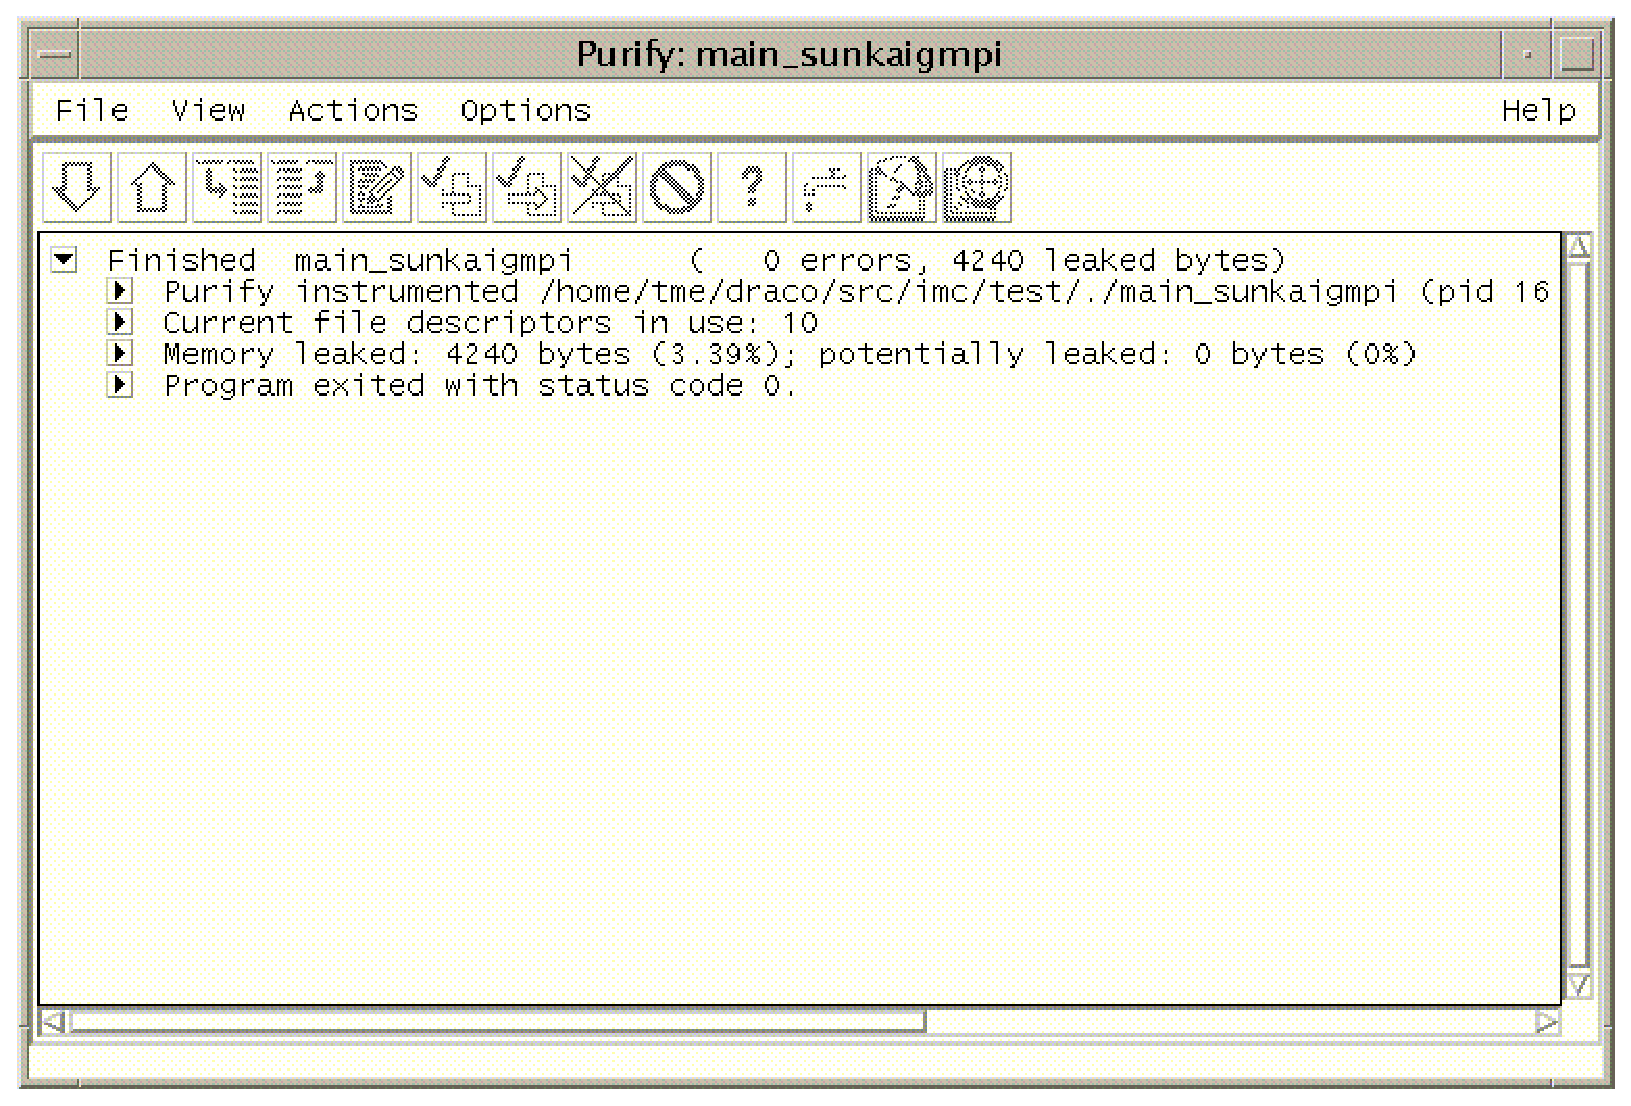
\includegraphics[width=4in]{main.eps}}
  \caption{\purify\ window for \dir{mpirun}.}
  \label{fig:main}
\end{figure}
second and third windows, Figs.~\ref{fig:proc}a and \ref{fig:proc}b, give
\begin{figure}
  \begin{center}
    \begin{tabular}{c}
      \subfigure[Processor 0
      window.]{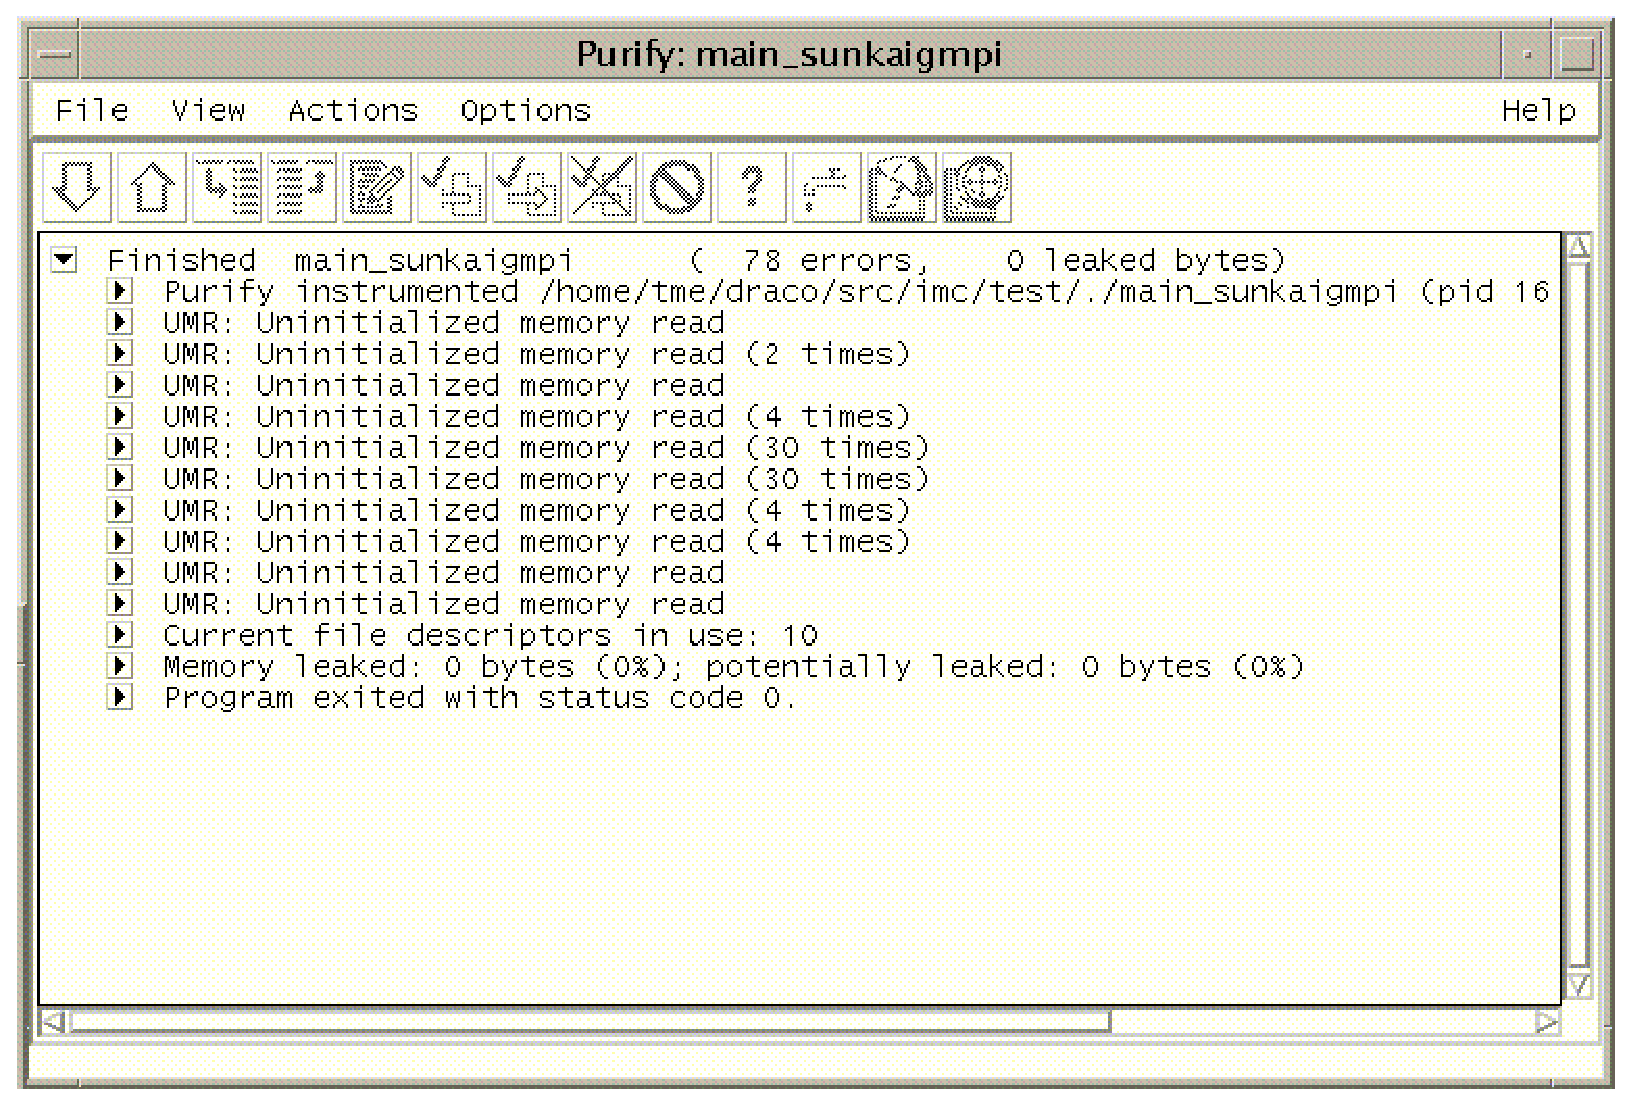
\includegraphics[width=4in]{p0.eps}} \\
      \subfigure[Processor 1
      window.]{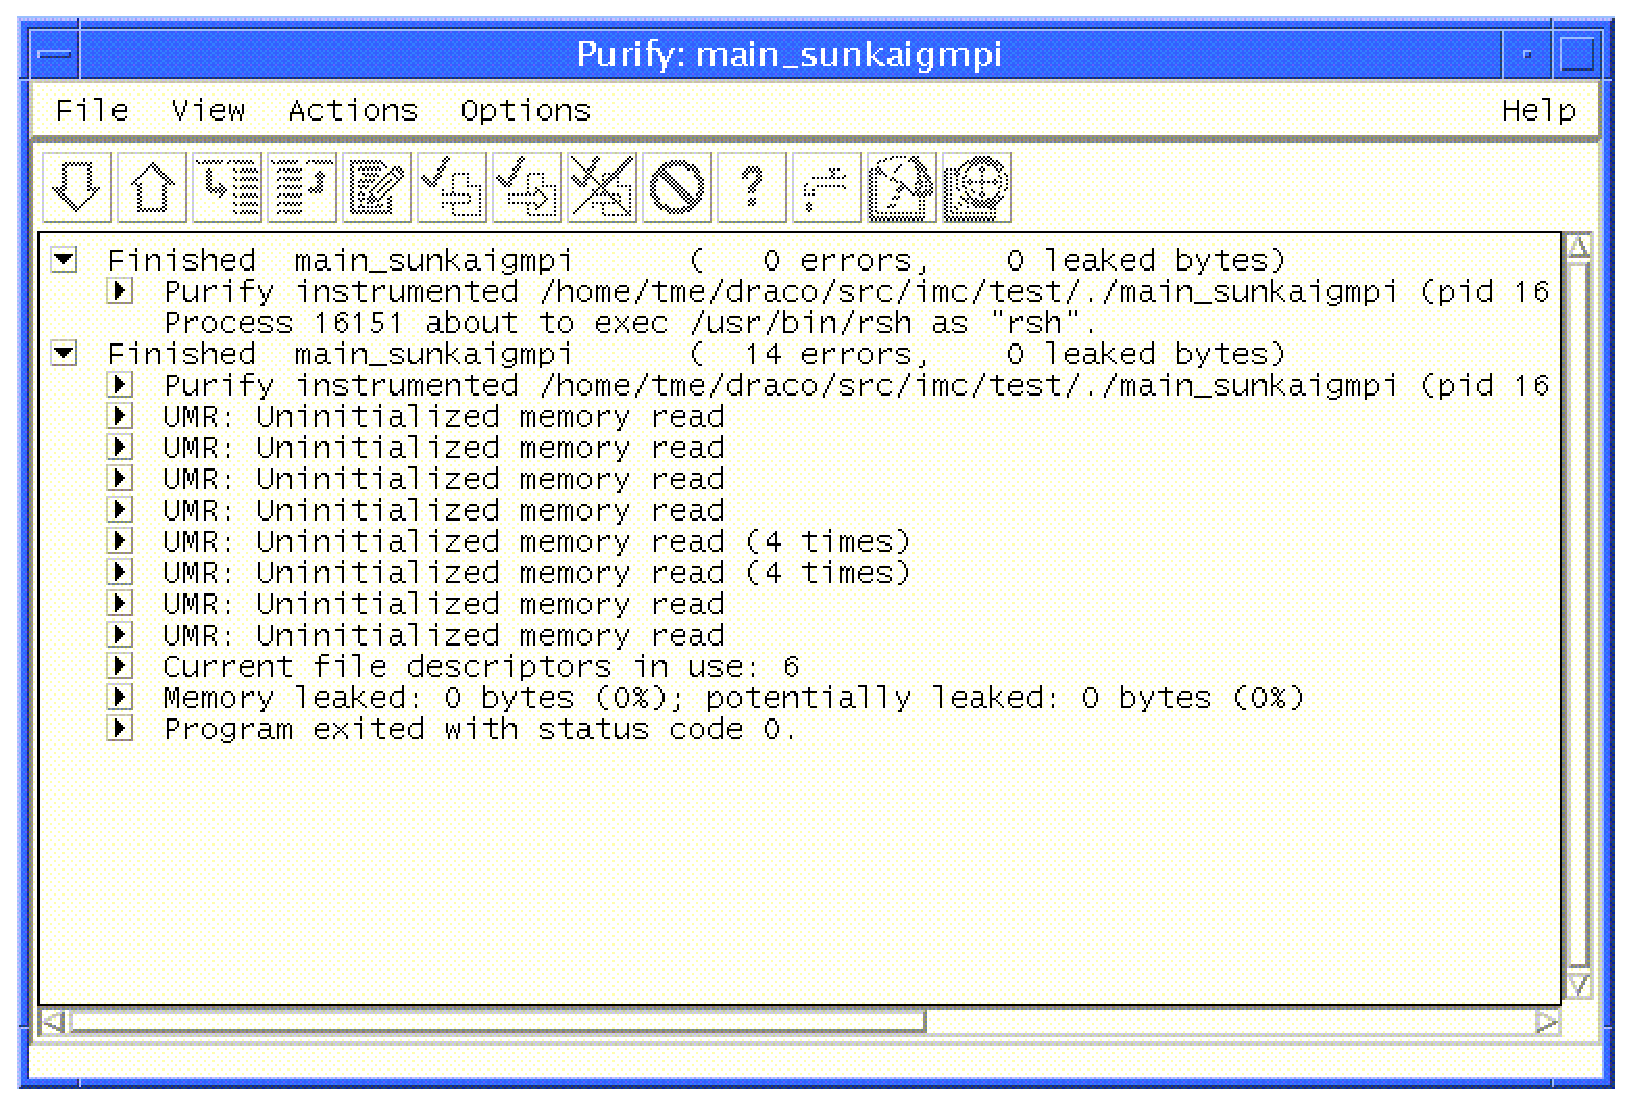
\includegraphics[width=4in]{p1.eps}}
    \end{tabular}
  \end{center}
  \caption{\purify\ windows for processors 0 and 1.}
  \label{fig:proc}
\end{figure}
diagnostics for the {\tt main\_sunkaigmpi} executable on processor 0
and 1, respectively.

The three windows show the following errors: Memory Leaks (MLK) in
Fig.~\ref{fig:main} and Unitialized Memory Reads (UMR) in
Figs.~\ref{fig:proc}a and b.  These errors are in the system files
\dir{rtlib} and \dir{libc}.  Thus, they will always be present and are
not part of the {\tt testp.cc} code.  Because these errors are part of
the system, we should suppress them in \purify.  The errors can be
permanently suppressed by making a {\tt .purify} file that contains
the following:
\begin{verbatim}
  suppress umr "libc.so.1"
  suppress mlk "rtlib.o"
\end{verbatim}
These suppression tags will prevent \purify\ from reporting UMR and
MLK errors that exist in \dir{libc} and \dir{rtlib}, respectively.
Thus, only errors that are part of the user-supplied code will appear
in the \purify\ windows.

%%---------------------------------------------------------------------------%%

\section*{Conclusions}

This memo has summarized the use of \purify\ in a parallel code
environment.  The examples are directed towards \C++ code compiled
with the \KCC\ compiler.  However, these methods should work with
other languages--{\tt F90}--and other compilers\footnote{Note that the
  link-line extension {\tt --link\_command\_prefix} is a \KCC\ command
  and will not work with other compilers.}.  In fact, Scott Turner
(XTM) has reported success using \purify\ with {\tt F90} on \dir{Blue
  Mountain}.  When running on \dir{Blue Mountain}, Turner reports that
unsetting the {\tt MPI\_DLOPEN} environment keeps \purify\ from
closing quickly if there is a MPI-node communication breakdown that
terminates the executable process.  See the MPI man-pages on \dir{Blue
  Mountain} for more information.

For more details about \purify, see the \purify\ manual~\cite{purify}
or man-page.

%%---------------------------------------------------------------------------%%

\section*{Acknowledgements}

The author thanks Scott Turner (XTM) for relating his experiences with 
\purify\ on \dir{ASCI Blue}.

%%---------------------------------------------------------------------------%%

\bibliographystyle{../tex/rnote}
\bibliography{../bib/draco}
 
\closing
\end{document}

%%---------------------------------------------------------------------------%%
%% end of 98099.tex
%%---------------------------------------------------------------------------%%
